\section*{2.1 The Skeleton of Primes: God Does Not Play Dice, God Composes Music}

\begin{figure}[h]
\centering
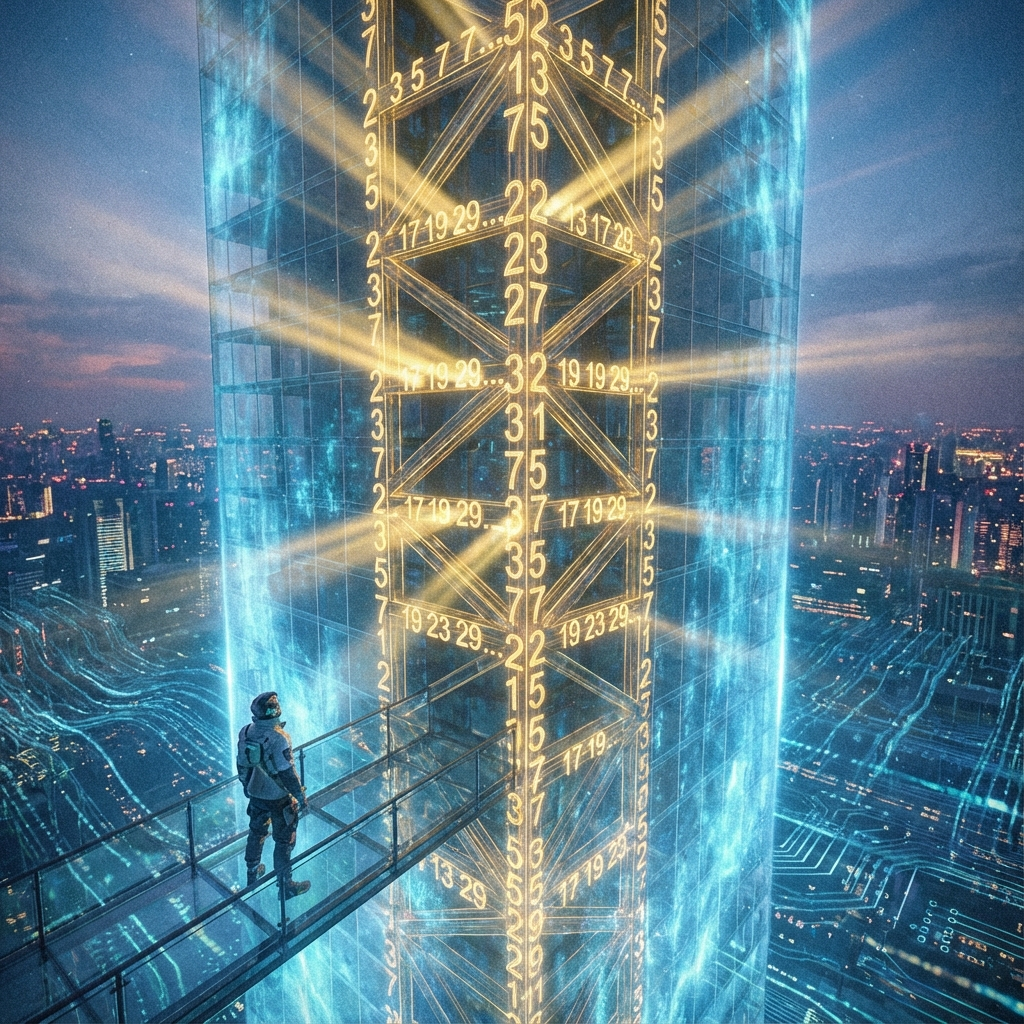
\includegraphics[width=0.8\textwidth]{assets/volume01-layer0-kernel-logic/chapter02-prime-skeleton-stairway/02-01-thematic.png}
\caption{Image}
\end{figure}

Albert Einstein once left a deafening quote to express his dissatisfaction with the intrinsic randomness in quantum mechanics: "God does not play dice." He firmly believed that behind those seemingly chaotic and fuzzy probability clouds, there must be a certain, elegant order, a rigid law yet to be discovered by us.

From the perspective of \textbf{HPA-ZΩ} theory, Einstein was right, but he was only half right. God indeed does not play dice, because playing dice is too low-level; that is a disordered piling of random numbers, unable to build such a precise and \textbf{Consistent} universe.

What is God doing? \textbf{God is composing music.}

When we peel away the layers of the material world, passing through molecules, atoms, quarks, and even passing through the quantum foam surging beneath, what do we actually see at the bottom layer of the universe (Layer 0)? We do not see hard particles, nor chaotic energy, but pure \textbf{Mathematical Structure}. More precisely, it is a rigid, unshakable system of \textbf{Prime Numbers}.

\textbf{1. The Only Rigidity in Chaos}

If you are an architect wanting to build an eternal building on a patch of flowing quicksand (quantum probability cloud), what do you need? You need to drive piles. You need to find some support points that are absolutely hard, absolutely unchanging with time, and unchanging with the observer's perspective, to maintain the structural \textbf{Consistency} of the entire building.

In the physical universe, such support points are actually hard to find. The speed of light bends at the edge of a black hole, time slows down in high-speed motion, and even mass itself is condensed energy. But in the mathematical universe, there is one thing that is absolutely rigid, and that is \textbf{Prime Numbers}: 2, 3, 5, 7, 11, 13, 17\ldots

Whether you are on Earth, or in the Andromeda Galaxy tens of billions of light-years away, or even in a parallel universe with completely different physical constants, 17 can essentially only be divisible by 1 and itself. The properties of prime numbers do not depend on physical laws, do not depend on the speed of light; they are a \textbf{Logical Necessity}.

Therefore, the operating system of this generative universe chose these \textbf{Prime Numbers} as the \textbf{"Load-bearing Wall"} or \textbf{"Prime Skeleton"} for constructing reality.

As we discussed in the previous chapter, the universe adopts a "lazy loading" mechanism to save computing power, allowing unobserved history to be in a fuzzy state. However, this fuzziness does not mean one can do whatever one wants. All generations and all retroactive corrections must be mounted on this \textbf{Prime Skeleton}. It ensures that even if reality is rendered in real-time, it remains as solid as a diamond.

\textbf{2. Hecke Dynamics: The Harmony of the Universe}

\begin{figure}[h]
\centering
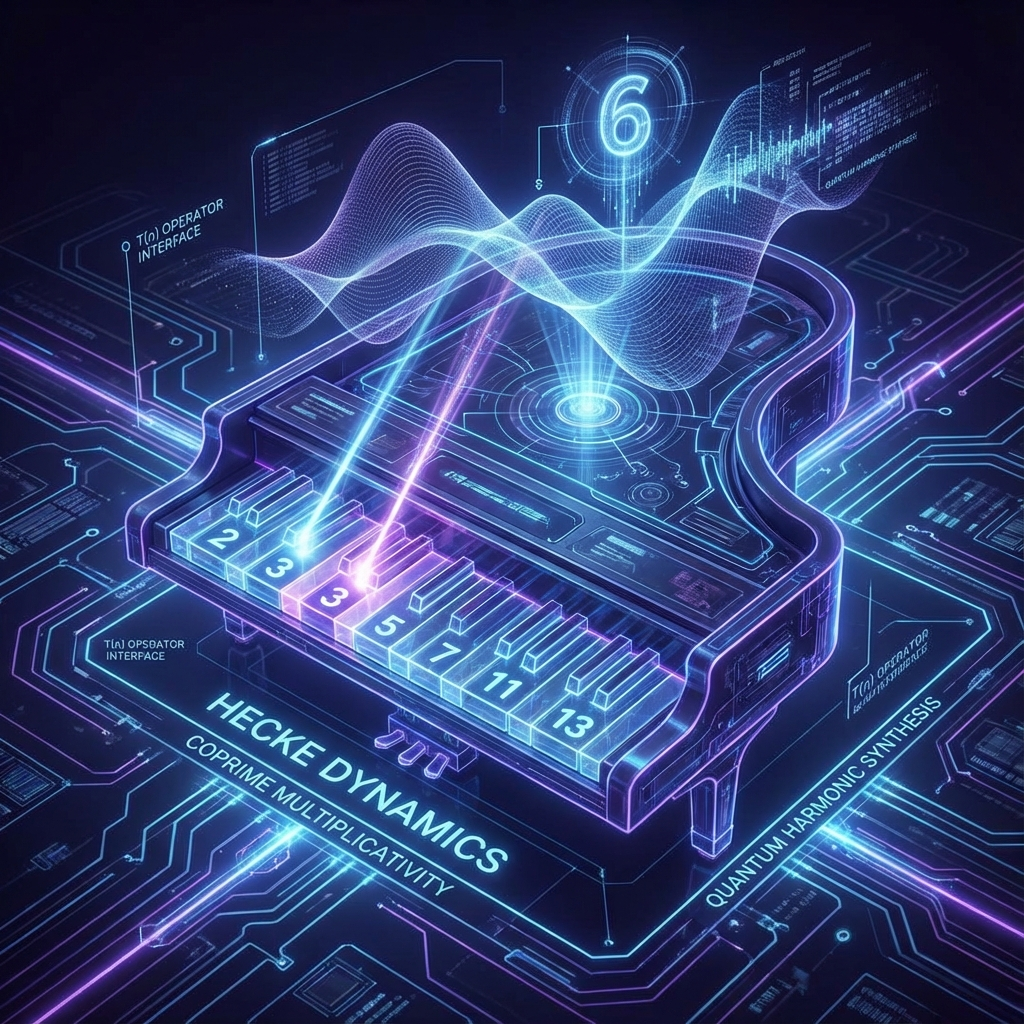
\includegraphics[width=0.8\textwidth]{assets/volume01-layer0-kernel-logic/chapter02-prime-skeleton-stairway/02-01-technical-1.png}
\caption{Image}
\end{figure}

In our theoretical model, this set of prime skeletons is not a static specimen. They generate resonance and interaction in this holographic universe through a mechanism called \textbf{"Hecke Operators"}.

To understand this abstract mathematical concept, let's go back to the metaphor of music.

Imagine the universe is a huge piano.

\begin{itemize}
\item \textbf{Prime Numbers (2, 3, 5\ldots)} are the \textbf{Strings} on this piano.
\item \textbf{Physical Reality} is the \textbf{Movement} produced by the vibration of the strings.
\item \textbf{Hecke Relations} are the strict \textbf{Rules of Harmony}.
\end{itemize}

Not all sound combinations are allowed. To maintain \textbf{Consistency}, the universe has set a strict algorithm: When you play the note "2" and the note "3", the background algorithm of the universe will automatically calculate the state of the note "6". This mechanism is mathematically called \textbf{"Coprime Multiplicativity"}.

This means that seemingly independent events in the universe are actually tightly locked by the prime skeleton in the deep layer. This strict mathematical constraint ensures that the universe does not collapse into a ball of harsh noise (logic crash) during the lazy loading process, but forms some kind of \textbf{"Eigenforms"} with high symmetry and stability.

This is why the electron orbits, crystal structures, and even the arrangement of flower petals (often following the Fibonacci sequence) we see are full of breathtaking geometric beauty. These beauties are not accidental; they are the \textbf{Projection} of the prime skeleton in the macroscopic world.

\textbf{3. Auto-completion System: Hum Your Vow}

\begin{figure}[h]
\centering
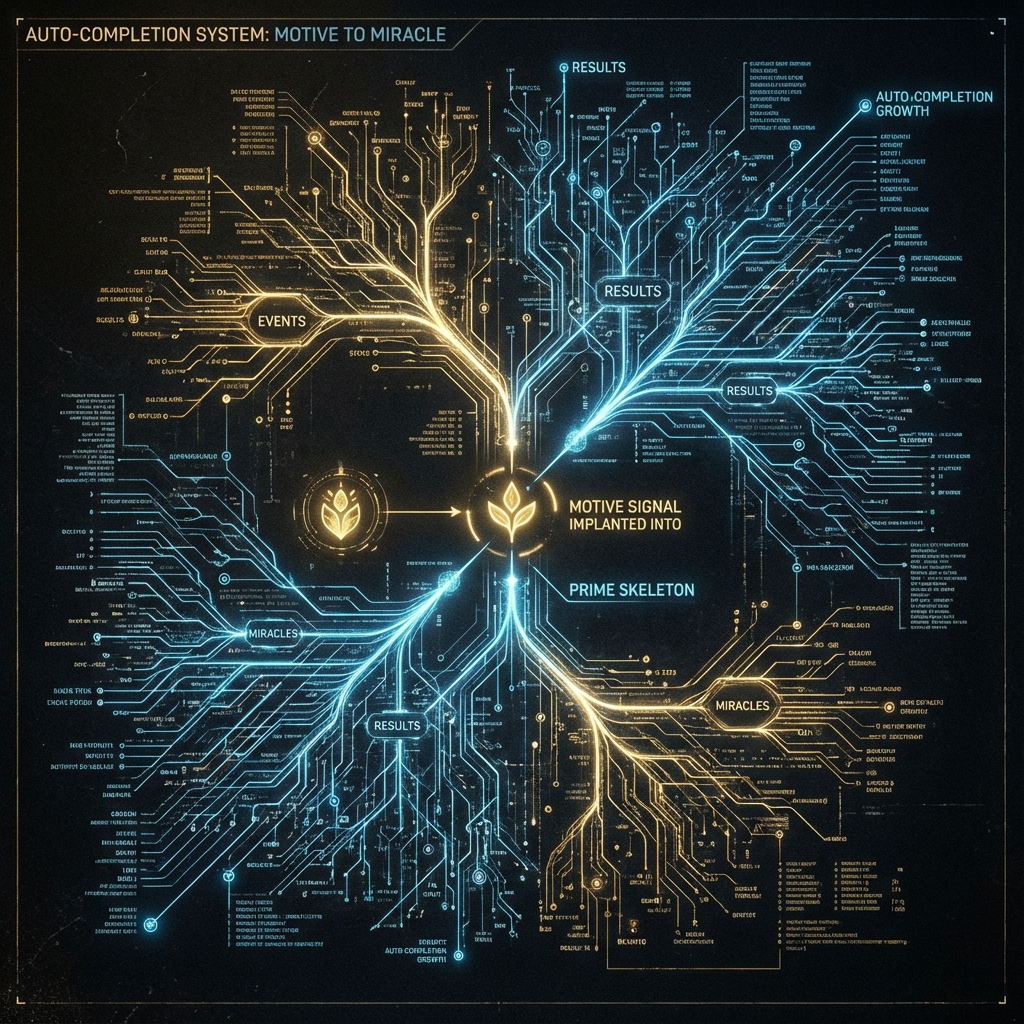
\includegraphics[width=0.8\textwidth]{assets/volume01-layer0-kernel-logic/chapter02-prime-skeleton-stairway/02-01-technical-2.png}
\caption{Image}
\end{figure}

Understanding the role of the prime skeleton, we can answer that core question: \textbf{"In this generative universe, how much power do we, as observers, actually possess?"}

Some New Age theories claim "what you think will manifest", which is inaccurate in physics. You cannot imagine a pink elephant appearing in the room out of thin air, because that violates the underlying physical logic and destroys the \textbf{Consistency} of the system.

However, \textbf{HPA-ZΩ} reveals a more subtle mechanism: \textbf{"Auto-completion"}.

Imagine you are using the "Hum to Search" function of a music player app, or using the auto-suggest function of a search engine. You don't need to input the score of the whole song, nor do you need to type out a complete article of thousands of words. You only need to hum \textbf{even two most critical notes}, or input \textbf{a few core keywords}.

As long as these few notes (keywords) are clear enough and strong enough, the system will automatically \textbf{Complete} the remaining melody for you based on the massive database and algorithmic logic.

In our universe:

\begin{itemize}
\item Those \textbf{Two Critical Notes} are your \textbf{"Vow" (Motive)}—the strong signal you send to the Dragon Pearl located at $i\infty$.
\item That massive \textbf{Database and Algorithm} are the \textbf{Prime Skeleton} and \textbf{Hecke Dynamics}.
\end{itemize}

When you send out a strong Vow consistent with the direction of truth (such as "I want to explore the truth of the universe"), you are actually plucking that deepest string. The inertial engine of the universe senses this vibration, and in order to maintain mathematical \textbf{Consistency} (to make this wish logically hold), it will follow the rigid skeleton of primes to \textbf{Automatically Generate} and \textbf{Retroactively Calculate} a series of complex opportunities, inspirations, coincidences, and material conditions to make this "symphony" complete.

You don't need to worry about every detail (such as "how that inspiration comes", "how to meet that person"); that is the work automatically calculated by the cosmic background (Layer 0) using \textbf{Hecke Relations}. You only need to ensure that your \textbf{"Main Melody" (Motive)} is clear and in tune.

This is the true meaning of \textbf{"God is composing music"}.

The universe is not a random casino, but a huge resonance box. Each of us is a performer. Although we cannot change the structure of the piano (physical laws/prime skeleton), we can choose which piece to play.

When we understand this, we understand: The so-called miracle is just the perfect \textbf{Resonance} between your \textbf{Vow Power} and the universe's underlying \textbf{Mathematical Skeleton}. In the next section, we will see how this piece of music climbs step by step from microscopic chaos to macroscopic truth along \textbf{"Jacob's Ladder"}.

